
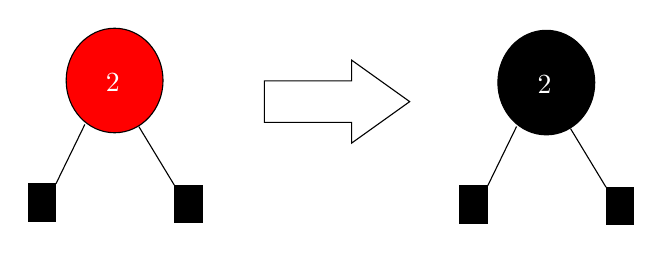
\begin{tikzpicture}[x=0.75pt,y=0.75pt,yscale=-1,xscale=1]
%uncomment if require: \path (0,706); %set diagram left start at 0, and has height of 706

\draw  [fill={rgb, 255:red, 0; green, 0; blue, 0 }  ,fill opacity=1 ]  (100.22, 253.65) rectangle (113.54, 271.61)   ;
\draw    (113.54,253.65) -- (127.5,225) ;


\draw  [fill={rgb, 255:red, 255; green, 0; blue, 0 }  ,fill opacity=1 ]  (141.83, 203.82) circle [x radius= 23.33, y radius= 25.18]  ;
\draw    (153.5,226) -- (170.62,254.26) ;


\draw  [fill={rgb, 255:red, 0; green, 0; blue, 0 }  ,fill opacity=1 ]  (170.62, 254.26) rectangle (183.94, 272.22)   ;
\draw  [fill={rgb, 255:red, 0; green, 0; blue, 0 }  ,fill opacity=1 ]  (308.22, 254.65) rectangle (321.54, 272.61)   ;
\draw    (321.54,254.65) -- (335.5,226) ;


\draw  [fill={rgb, 255:red, 0; green, 0; blue, 0 }  ,fill opacity=1 ]  (349.83, 204.82) circle [x radius= 23.33, y radius= 25.18]  ;
\draw    (361.5,227) -- (378.62,255.26) ;


\draw  [fill={rgb, 255:red, 0; green, 0; blue, 0 }  ,fill opacity=1 ]  (378.62, 255.26) rectangle (391.94, 273.22)   ;
\draw   (214,204) -- (256,204) -- (256,194) -- (284,214) -- (256,234) -- (256,224) -- (214,224) -- cycle ;

\draw (141,205) node [color={rgb, 255:red, 255; green, 255; blue, 255 }  ,opacity=1 ] [align=left] {2};
\draw (349,206) node [color={rgb, 255:red, 255; green, 255; blue, 255 }  ,opacity=1 ] [align=left] {2};


\end{tikzpicture}